\chapter{Evaluation} \label{chap:evaluation} \minitoc

\section*{}

This section evaluates how the solution developed proves the hypothesis proposed in Chapter \ref{chap:problem_statement}.

\textcolor{blue}{Complete...}

% First, an explanation of the scenarios will be made, as well as their relation to the features developed and their advantages. 

\section{Scenarios and Experiments}\label{sec:scenarios_experiments}

The testing of the proposed solution diverged in two different scenarios. The first simulates physical devices with the use of Docker containers running the Unix port of micropython, allowing the construction of scalable scenarios with minimal costs. The second scenario uses physical devices, such as ESP8266 and ESP32, connected to the same Wi-Fi.

\begin{enumerate}
    \item A room has 3 sensors that give temperature and humidity readings every minute. There’s a virtual sensor that compares the results (of both temperature and humidity) and triggers depending on some configured thresholds. An AC uses those readings to decide (a) if it switches on/off, (b) its operating mode: cool, heat, and dehumidify. The Minimal Working System (MWS) consists in (a) one temperature sensor, (b) one humidity sensor, (c) one node capable of making the decision, and (d) working communication channels amongst them.
    \item 20 devices, where each device redirects its input to its output. \textcolor{red}{improve}
\end{enumerate}

The first scenario aims to test the features of the developed solution with a moderately simple Node-RED flow, taking advantage of the nodes developed for micropython code generation support. The second scenario allows the comparison of the developed solution to the already existing solutions.

\textcolor{red}{Refactor this enumeration, with some explaining of some terms}

\textbf{Scenario 1}:
\begin{enumerate}
    \item \textbf{Sanity check.} All tasks are simple readings and forwarding, no compensation or other fault-tolerance strategy. Each sensor does its own thing. Orchestration is centralized. We expect all roundtrips to take less than the smallest part that can be resolved (measurement capability, which we estimate to be <1s).
    \item \textbf{Re-orchestration.}
        \begin{itemize}
            \item \textbf{Experiment A.} MWS is achieved via multiple possible configurations by selective (provoked) device failure (fail-stop);
            \item \textbf{Experiment B.} Inconsistent device behaviour, e.g. appear and disappear in shorter intervals lower that the time needed for orchestrating convergence (OCT), that leads to activity impacting the MWS;
            \item \textbf{Experiment C.} With 20 devices, each one with different processing capabilities. During orchestration, some devices will develop an out-of-memory error because they can't process all the processing tasks assigned to them, specifically the size of the script given. The orchestrator decides to send less tasks to these devices. The system will converge in a working solution. \textit{This scenario will be implemented with a modified device script. When devices receive a script, it will generate a memory error if the length of the script passes a certain threshold. This simulates the memory constraints of devices when receiving a file to big.}
            \item \textbf{Experiment D.} With 20 devices, some of them have a memory leak with an unknown cause. After random time Random(t0,t1), these problematic devices stop working with an out-of-memory error. The orchestrator thinks that the devices can't handle the quantity of processing tasks assigned to them, so in the re-orchestration it will assign fewer tasks. Since these devices will always break, the orchestrator will eventually not consider these devices in the assignment of nodes. \textit{This scenario will be implemented with a modified device script that will trigger an out-of-memory error after a random period after executing the given tasks.}
            \item \textbf{Experiment E.} With 20 devices, there is a device that is sensitive to a particular node, which causes the device to give out an out-of-memory error. The orchestrator will potentially assign this node to the specific device. When the device gives out the out-of-memory error, the orchestrator will eventually converge in a solution where the node is not assigned to the particular device, and the system will converge.  \textit{These out-of-memory errors will be simulated with the use of a failure node that forces an \texttt{MemoryException} in the device.}
        \end{itemize}
        Verifies that:
        \begin{enumerate}
            \item \textbf{Restrictions (predicates) are enforced.} Check that possible configurations lead to solutions that enforce defined predicates;
                \begin{enumerate}
                    \item Temperature and humidity might coexist in the same, or in dedicated, devices;
                \end{enumerate}
            \item \textbf{Priorities are honored.} Check that all specified priorities were taken into account, and only violated if necessary;
                \begin{enumerate}
                    \item Priority is given to edge devices, but fog and cloud can be used;
                    \item Priority is given to the maximum level of decentralization, but some centralization can be used.
                \end{enumerate}
        \end{enumerate}
    \item \textbf{Latency.} Make devices selectively slow and check the consequences; might impact OCT and MWS. ? \textcolor{red}{was not implemented}
\end{enumerate}

\textbf{Scenario 2}:
With the use of 20 physical devices, both ESP8266 and ESP32, implement a line topology, where a message is sent to a starting device, that will propagate it to its output. All the devices implement this propagation logic, which results in the initial message reaching the end of the line. The propagation time is measured, starting when the message is sent and ending when the message reaches the last node.
This experience is implemented in several environments:
\begin{enumerate}
    \item \textbf{Node-RED original}. Runs the experiment in the original Node-RED, using the default option (events) as the communication channel between nodes.
    \item \textbf{Node-RED + MQTT}. Run the experiment in Node-RED, using MQTT as the communication channel between nodes.
    \item \textbf{Node-RED modified + Dockers (same host)} Runs the experiment in the modified version of Node-RED, with each node assigned to a different virtual device, running in a Docker container. The virtual devices are in the same host machine running the MQTT server instance.
    \item \textbf{Node-RED modified + Dockers (different host)} Runs the experiment in the modified version of Node-RED, with each node assigned to a different virtual device, running in a Docker container. The MQTT server instance is in a different host machine from the one running the virtual devices. All machines are connected through Wi-Fi.
    \item \textbf{Physical + MQTT} Runs the experiment in physical devices without the developed firmware. Each device runs a simple micropython script that executes the wanted behaviour, communicating by MQTT. No Node-RED is used.
    \item \textbf{Node-RED modified + MQTT + Physical + Firmware} Runs the experiment with the developed solution, with each node assigned to a different physical device running the developed micropython firmware. All communicating is made using MQTT.
\end{enumerate}

\section{Discussion}\label{sec:evaluation_discussion}

\textcolor{blue}{For each experiment, analyse the data and discuss the results - many graphs, more tables and lots of text - fun times and very little time!}

\subsection{Scenario 1}\label{sec:discussion_scenario1}

\textcolor{blue}{Talk about the results of the scenario1 experiments, with graphs, prints of the scenario in Node-RED and conclusions}

\subsection{Scenario 2}\label{sec:discussion_scenario2}

As mentioned previously, several experiences were made to compare the developed solution to existing ones. To this end goal, a simple experiment of passing a message through several devices was implemented and the time the message takes to pass through all the devices was measured. The implementation of the scenario in the Node-RED tool is shown in Figure \ref{fig:scenario2_node_red}. The \textit{nothing} nodes execution consists of only redirecting their input to their output. The message consisting of the current timestamp is inserted into the system by the \textit{inject} node with user input, and the same message is showcased by the \textit{debug} node, the green one.

\begin{figure}[h]
\centering
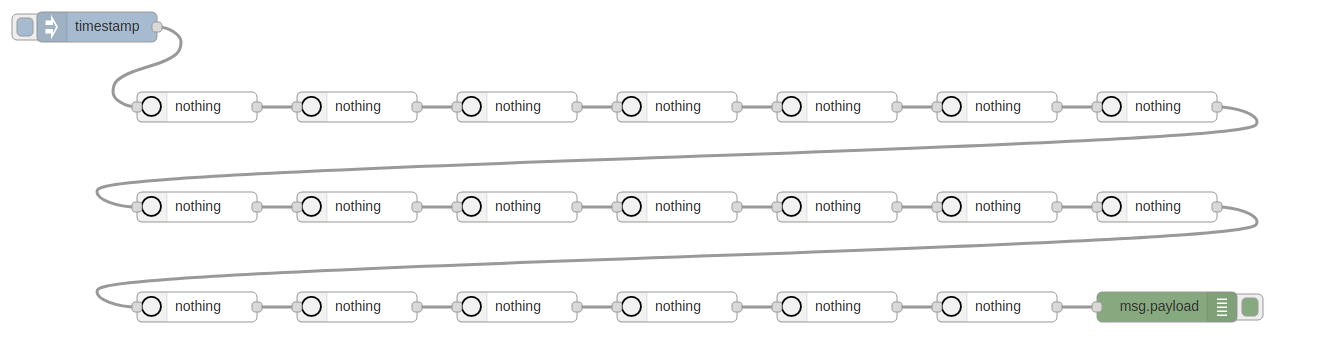
\includegraphics[width=\textwidth]{scenario2.png}
\caption[Solution's overview]{Node-RED implementation of scenario 2}\label{fig:scenario2_node_red}
\end{figure}

This same setup was replicated in several environments, as mentioned before. Each experiment was replicated 10 times, resulting in the data seen in Table \ref{tab:scenario2_table} and visually detailed in Figure \ref{fig:scenario2_candlestick}.

\captionsetup{belowskip=12pt,aboveskip=4pt}
\begin{table}[ht]
    \centering
    \resizebox{0.8\textwidth}{!}{%
    \begin{tabular}{ l  c  c  c  c }
        \toprule
        \textbf{Label} & \textbf{Min} & \textbf{Q2} & \textbf{Q3} & \textbf{Max}\\
        \midrule
        Node-RED original & 3 & 10 & 13.25 & 15 \\
        Node-RED + MQTT & 134 & 430.5 & 711.25 & 883 \\
        Node-RED modified + Dockers (same host) & 1217 & 1318 & 1573.75 & 1665 \\
        Node-RED modified + Dockers (different host) & 1445 & 2536 & 2708 & 3059 \\
        Physical + MQTT & 3616 & 4142 & 4372 & 4452 \\
        Node-RED modified + MQTT + Physical + Firmware & 4168 & 4569 & 5087.75 & 5940 \\
        \bottomrule
    \end{tabular}
    }
    \caption{Scenario 2 results}
    \label{tab:scenario2_table}
\end{table}{}

\begin{figure}[h]
\centering
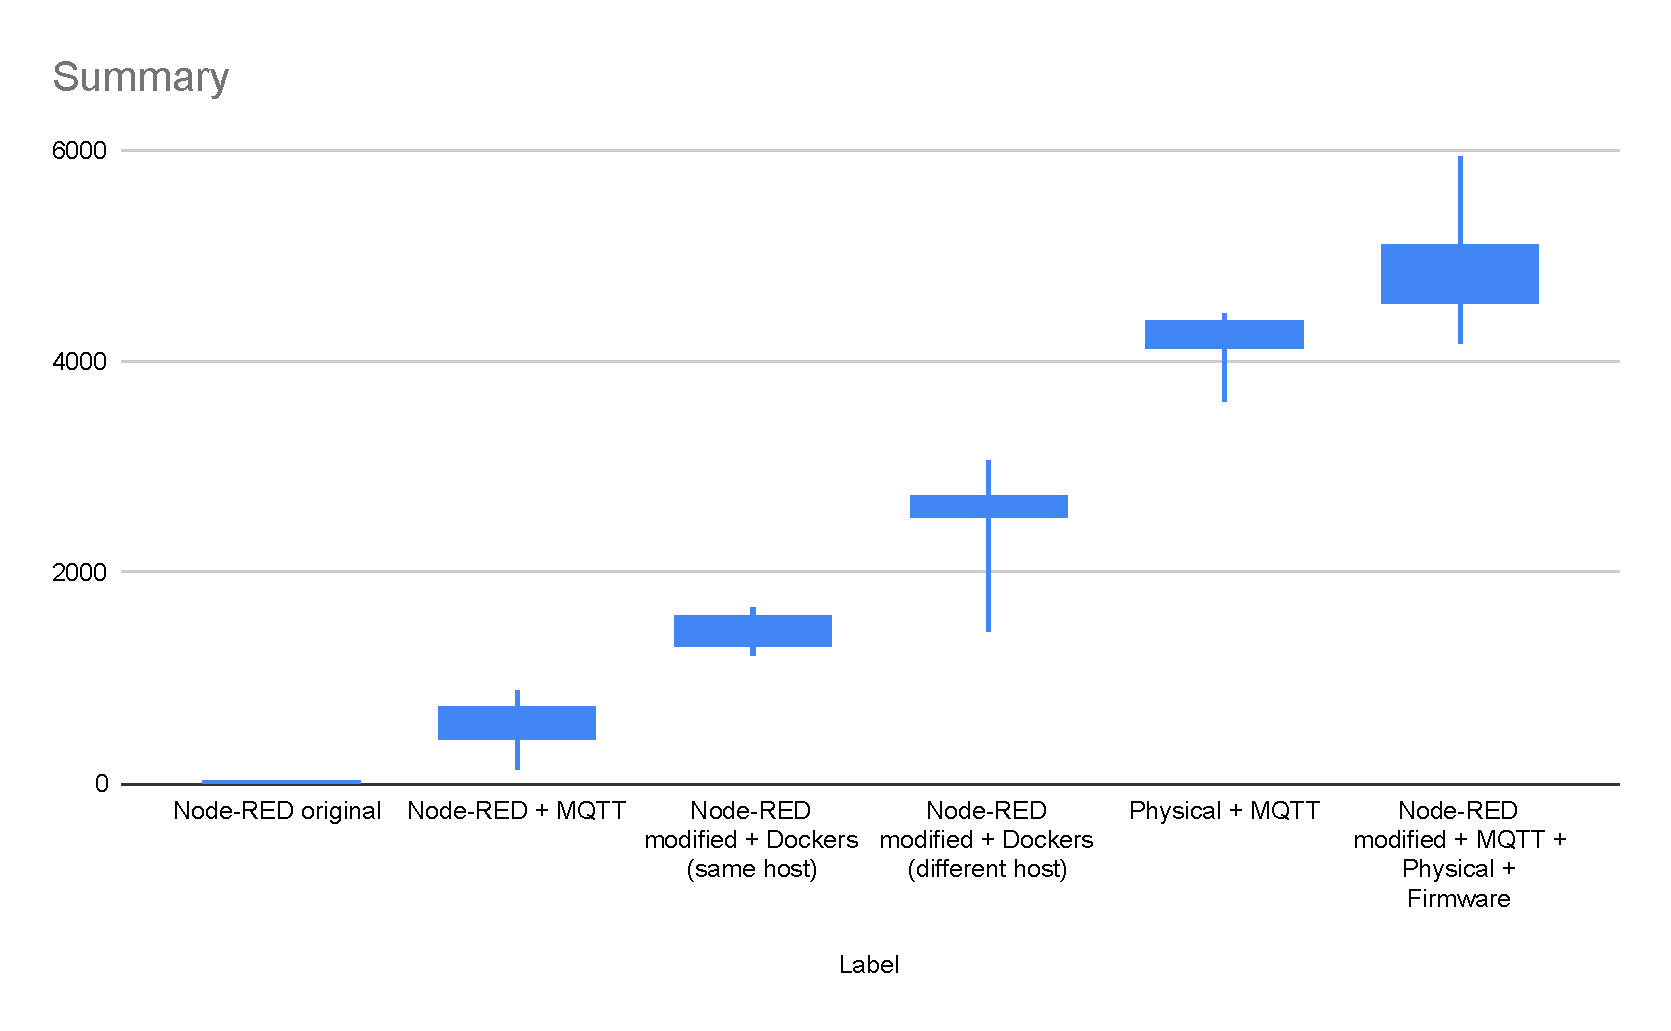
\includegraphics[width=\textwidth]{scenario2_graph.pdf}
\caption[Scenario 2 results]{Scenario 2 results}\label{fig:scenario2_candlestick}
\end{figure}

With the given results, we can conclude several things. 

\textcolor{blue}{Talk about how the communication stack hinders the speed of the solution - aka, different host, as well as the micropython firmware also hinders}

\textcolor{red}{Add other tables with the timestamps in the annex}

\subsection{Overview}\label{sec:discussion_overview}

\textcolor{blue}{Overview of the evaluation of the system, with conclusions of the evaluation of the system as a whole}

\section{Conclusions}\label{sec:evaluation_conclusions}

